\section{Diagram Alir Metodologi}
\label{sec:diagram-alir}
 
\noindent Penelitian dimulai dengan meninjau metrik lubang hitam Schwarzschild sebagai fondasi
dasar sistem fisis yang digunakan. Penelitian menerapkan metrik ini pada dua latar
belakang ruang-waktu yang berbeda, yaitu latar belakang Schwarzschild tak hingga datar ($\Lambda = 0$)
dan latar belakang Schwarzschild Anti-de Sitter
($\Lambda < 0$). Setelah metrik pada masing-masing latar belakang terdefinisi,
metrik diinjeksikan ke dalam persamaan master perturbasi medan skalar \eqref{eq:appkg-takbermassa} untuk memodelkan
dinamika perturbasi medan skalar terhadap lubang hitam Schwarzschild di kedua latar belakang.
 
Dari persamaan master yang diperoleh, penelitian membagi kajian menjadi dua kasus, yaitu medan skalar tak bermassa dan medan skalar bermassa. Kedua kasus ini menghasilkan potensial efektif yang berbeda dalam
persamaan master, namun prosedur penyelesaian tetap menggunakan alur metode yang sama. Pada setiap
kasus, dilakukan analisis kondisi batas radial yang sesuai dengan masing-masing latar
belakang. Setelah kondisi batas telah ditentukan, solusi radial dikonstruksi menggunakan
ansatz deret Frobenius yang mengekspansi fungsi gelombang di sekitar cakrawala
peristiwa. Substitusi ansatz ini ke dalam persamaan master menghasilkan relasi rekurensi
linear bersuku banyak yang kemudian direduksi menjadi relasi rekurensi tiga suku melalui
metode eliminasi Gauss. Relasi rekurensi tiga suku sebagai syarat untuk dapat dilakukan perhitungan menggunakan
metode pecahan berlanjut hingga didapatkan nilai frekuensi \textit{quasinormal modes} ($\omega$). Setelah hasil frekuensi pada setiap latar belakang
didapatkan, penelitian memasuki tahap analisis hasil dan pembahasan untuk mendapatkan jawaban atas permasalahan dan tujuan
yang direncanakan. Alur logika penelitian ini secara ringkas digambarkan dalam diagram alir
pada Gambar~\ref{fig:flowchart}.
 
\newpage
 
\begin{figure}[htbp]
\centering
% Ubah 'nama_file_gambar.png' sesuai dengan nama file gambarmu yang ada di dalam folder yang sama
% Kamu bisa mengubah nilai 0.8 untuk memperbesar atau memperkecil ukuran gambar
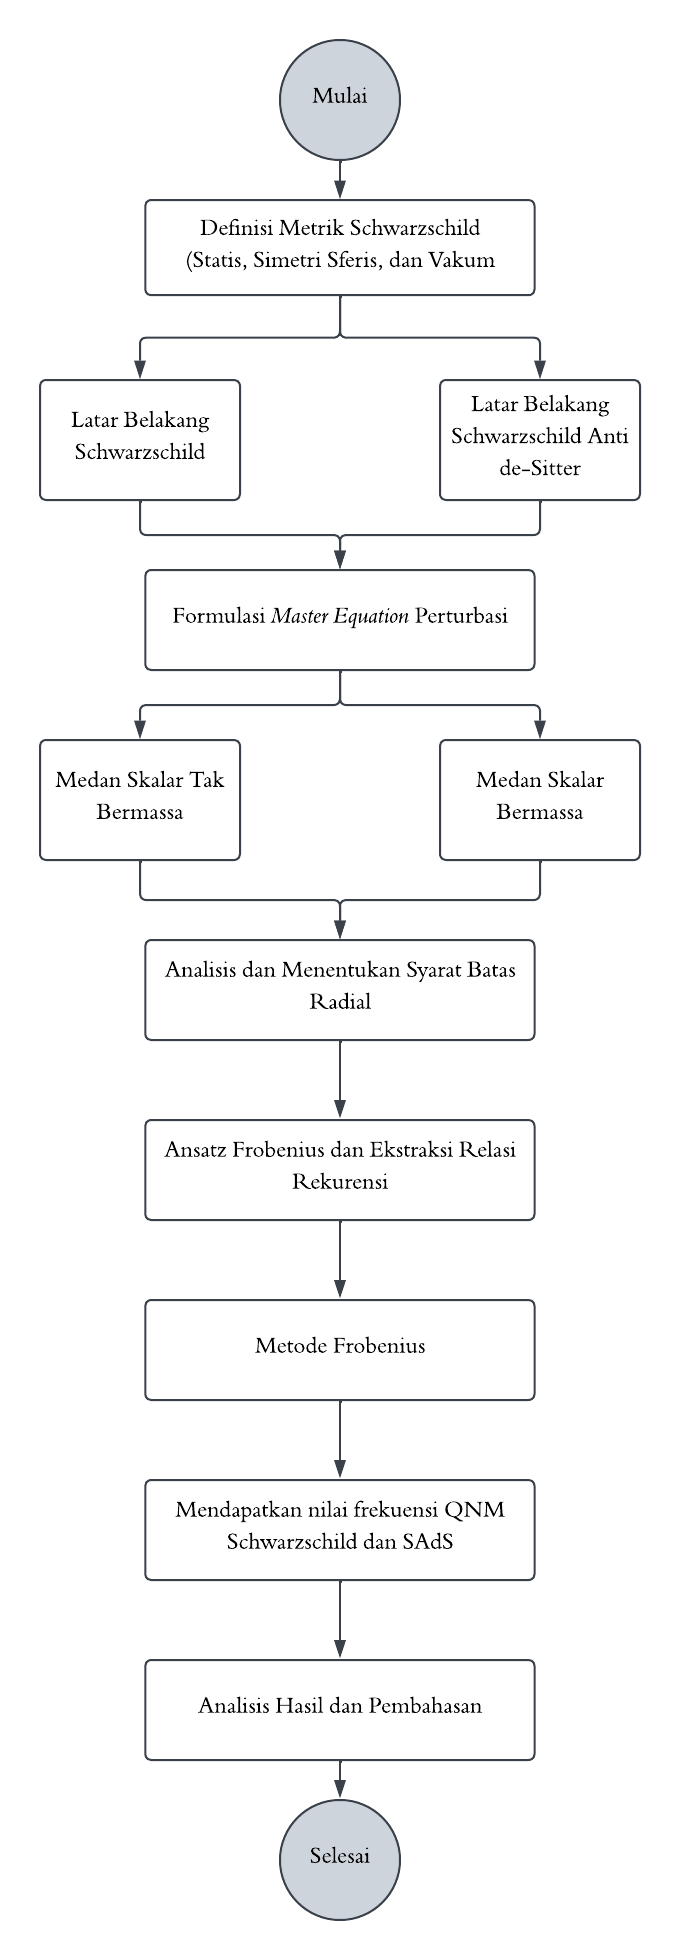
\includegraphics[width=0.4\textwidth]{uploads/dialir.png}
\caption{Diagram Alir Metodologi Penelitian Mode Kuasinormal}
\label{fig:flowchart}
\end{figure}